\documentclass[notes]{subfiles}
\begin{document}
	\addcontentsline{toc}{section}{1.10 - Logistic Functions \& Models}
	\fancyhead[RO,LE]{\bfseries  \large \nameref{cs110}} 
	\fancyhead[LO,RE]{\bfseries \currentname}
	\fancyfoot[C]{{}}
	\fancyfoot[RO,LE]{\large \thepage}	%Footer on Right \thepage is pagenumber
	\fancyfoot[LO,RE]{\large Chapter 1.10}


\section*{Logistic Functions \& Models}\label{cs110}
	\subsection*{Logistic Functions}
		A logistic has the following descriptions:\\
		\begin{itemize}
			\item \underline{Algebraically}: A logistic model has an equation of the form \showto{ins}{\fbox{$f(x) = \dfrac{c}{1+ae^{bx}}$}}\showto{st}{\blank{2}} where \showto{st}{\\[15pt]} $a,b\neq 0$ are constants, and $c > 0$ is the \showto{ins}{\fbox{carrying capacity/limiting value}}\showto{st}{\blank{3}}.  \\
			\item \underline{Graphically}: See below; logistics have two horizontal asymptotes at \showto{ins}{\fbox{$y=0,y=c$}}\showto{st}{\blank{1.85}}.  
		\end{itemize}

	\subsection*{Logistic Models}
		For logistic models, we have the following information:
		\begin{figure}[h!]
		\fbox{
		\begin{minipage}{1in}
		\centering
			$\underline{b > 0}$\\
			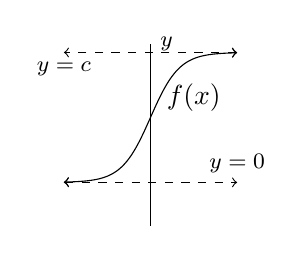
\begin{tikzpicture}[x = .55cm, y = .55cm]
				\draw[<->,dashed] (-2,0)--(2,0) node[above] {\footnotesize $y = 0$}; %x-axis / asymptote
				\draw[<->,dashed] (2,3)--(-2,3) node[below] {\footnotesize $y = c$}; %y = c asymptote
				\draw (0,-1)--(0,3.2) node[right] {\footnotesize $y$}; %y-axis
				\draw[<->, smooth, samples = 100, domain = -2.:2.] plot (\x, {3/(1 + exp((-3)*\x))});	
				\draw (1,2.5) node[below] {$f(x)$};
			\end{tikzpicture}	
		\end{minipage}
		\begin{minipage}{2in}
		\begin{itemize}
			\item $\ds \lim_{x\to\infty} f(x) = $ \showto{ins}{\fbox{$c$}}\showto{st}{}
			\item $\ds \lim_{x\to -\infty} f(x) = $ \showto{ins}{\fbox{0}}\showto{st}{}
			\item $f$ is always \showto{ins}{\fbox{increasing}}\showto{st}{}
			\item $f$ is \showto{ins}{\fbox{concave up then down}}\showto{st}{}
		\end{itemize}
		\end{minipage}
		}
		\fbox{
		\begin{minipage}{1in}
		\centering
		$\underline{b < 0}$\\
			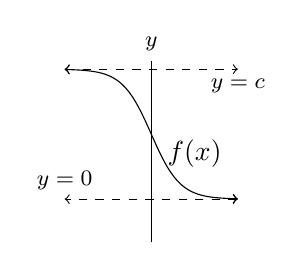
\begin{tikzpicture}[x = .55cm, y = .55cm]
				\draw[<->,dashed] (2,0)--(-2,0) node[above] {\footnotesize $y = 0$}; %x-axis / asymptote
				\draw[<->,dashed] (-2,3)--(2,3) node[below] {\footnotesize $y = c$}; %y = c asymptote
				\draw (0,-1)--(0,3.2) node[above] {\footnotesize $y$}; %y-axis
				\draw[<->, smooth, samples = 100, domain = -2.:2.] plot (\x, {3/(1 + exp((3)*\x))});	
				\draw (1,.5) node[above] {$f(x)$};
			\end{tikzpicture}
		\end{minipage}
		\begin{minipage}{2in}
			\begin{itemize}
				\item $\ds \lim_{x\to\infty} f(x) = $ \showto{ins}{\fbox{$0$}}\showto{st}{}
				\item $\ds \lim_{x\to -\infty} f(x) = $ \showto{ins}{\fbox{$c$}}\showto{st}{}
				\item $f$ is always \showto{ins}{\fbox{decreasing}}\showto{st}{}
				\item $f$ is \showto{ins}{\fbox{concave down then up}}\showto{st}{}
			\end{itemize}
		\end{minipage}
		}
		\end{figure}
		\newpage

	\subsection*{Examples}
		\begin{ex} The number of NBA players taller than a given height are listed in the table below.
			\begin{center}
				{\renewcommand{\arraystretch}{1.2}
				\begin{tabular}{|c|c||c|c|}\hline
					\textbf{Height} (in inches) & \textbf{Number of Players} & \textbf{Height} (in inches) & \textbf{Number of Players} \\ \hline
					68'' & 490 & 80'' & 203 \\ \hline
					70'' & 487 & 82'' & 86 \\ \hline
					72'' & 467 & 84'' & 13 \\ \hline
					74'' & 423 & 86'' & 2 \\ \hline
					76'' & 367 & 88'' & 1 \\ \hline
					78'' & 293 &  &  \\ \hline
				\end{tabular}
				}
			\end{center}
			\begin{enumerate}[(a)]
				\item Using the scatterplot, explain why a logistic model is best for this data.
					\vs{.5}
				\item Align the data so that 68'' corresponds to an input of 0, and find the complete logistic model.
					\vs{1}
				\item Describe (using limit notation) the end behavior of the model as height increases.
					\vs{.75}
			\end{enumerate}
		\end{ex}
			\newpage

		\begin{ex}
			The narrow band residential internet access, as a percentage of total residential internet access, is given below.
			\begin{center}
				{\renewcommand{\arraystretch}{1.2}
				\begin{tabular}{|c|c||c|c|} \hline
					\textbf{Year} & \textbf{Narrow Band Users} (in \%) & \textbf{Year} & \textbf{Narrow Band Users} (in \%) \\ \hline
					2000 & 89.4 & 2008 & 9.6 \\ \hline
					2001 & 80.7 & 2009 & 7.3 \\ \hline
					2002 & 70.9 & 2010 & 4.3 \\ \hline
					2003 & 58.3 & 2011 & 3.0 \\ \hline
					2004 & 45.9 & 2012 & 2.5 \\ \hline
					2005 & 35.3 & 2013 & 1.5 \\ \hline
					2006 & 21.5 & 2014 & 1.0 \\ \hline
					2007 & 12.2 & & \\ \hline
				\end{tabular}
				}
			\end{center}
			\begin{enumerate}[(a)]
				\item Based on the scatterplot, explain why a logistic model is best.
					\vs{.5}
				\item Align the model so that 2000 corresponds to an input of 0.  Find the complete logistic model for the data.
					\vs{1}
				\item Write the equations for the two asymptotes.
					\vs{.5}
				\item Estimate the location of the inflection point
					\vs{.5}
			\end{enumerate}
		\end{ex}
	\clearpage
\end{document}